%% Based on a TeXnicCenter-Template, which was
%% created by Christoph B�rensen
%% and slightly modified by Tino Weinkauf.
%%%%%%%%%%%%%%%%%%%%%%%%%%%%%%%%%%%%%%%%%%%%%%%%%%%%%%%%%%%%%

\documentclass[a4paper,12pt]{scrartcl} %This is a special class provided by the KOMA script, which does a lot of adjustments to adapt the standard LaTeX classes to european habits, change to [a4paper,12pt,twoside] for doublesided layout


%########################### Preferences #################################


% ******** vmargin settings *********
\usepackage{vmargin} %This give you full control over the used page arae, it maybe not the idea od Latex to do so, but I wanted to reduce to amount of white space on the page
\setpapersize{A4}
\setmargins{3.5cm}%			%linker Rand, left edge
					 {1.5cm}%     %oberer Rand, top edge
           {14.7cm}%		%Textbreite, text width
           {23.42cm}%   %Texthoehe, text hight
           {14pt}%			%Kopfzeilenh�he, header hight
           {1cm}%   	  %Kopfzeilenabstand, header distance
           {0pt}%				%Fu�zeilenhoehe footer hight
           {2cm}%    	  %Fusszeilenabstand, footer distance         

% ********* Font definiton ************
\usepackage{t1enc} % as usual
\usepackage[latin1]{inputenc} % as usual
\usepackage{times}		
%\usepackage{mathptmx}  	%mathematical fonts for use with times, I encountered some problems using this package togather with pdftex, which I was not able to resolve

% ********* Graphics definition *******
\usepackage[pdftex]{graphicx} % required to import graphic files
\usepackage{color} %allows to mark some entries in the tables with color
\usepackage{eso-pic} % these two are required to add the little picture on top of every page
\usepackage{everyshi} % these two are required to add the little picture on top of every page
\renewcommand{\floatpagefraction}{0.7} %default:0.5 allows two big pictures on one page

%********** Enybeling Hyperlinks *******
\usepackage[pdfborder=000,pdftex=true]{hyperref}% this enables jumping from a reference and table of content in the pdf file to its target

% ********* Table layout **************
\usepackage{booktabs}	  	%design of table, has an excellent documentation
%\usepackage{lscape}			%use this if you want to rotate the table together with the lines around the table

% ********* Caption Layout ************
\usepackage{ccaption} % allows special formating of the captions
\captionnamefont{\bf\footnotesize\sffamily} % defines the font of the caption name (e.g. Figure: or Table:)
\captiontitlefont{\footnotesize\sffamily} % defines the font of the caption text (same as above, but not bold)
\setlength{\abovecaptionskip}{0mm} %lowers the distace of captions to the figure


% ********* Header and Footer **********
% This is something to play with forever. I use here the advanced settings of the KOMA script

\usepackage{scrpage2} %header and footer using the options for the KOMA script
\renewcommand{\headfont}{\footnotesize\sffamily} % font for the header
\renewcommand{\pnumfont}{\footnotesize\sffamily} % font for the pagenumbers

%the following lines define the pagestyle for the main document
\defpagestyle{cb}{%
(\textwidth,0pt)% sets the border line above the header
{\pagemark\hfill\headmark\hfill}% doublesided, left page
{\hfill\headmark\hfill\pagemark}% doublesided, right page
{\hfill\headmark\hfill\pagemark}%  onesided
(\textwidth,1pt)}% sets the border line below the header
%
{(\textwidth,1pt)% sets the border line above the footer
{{\it Documentation for Alevin Developers}\hfill }% doublesided, left page
{\hfill{\it Documentation for Alevin Developers}}% doublesided, right page
{\hfill{\it Documentation for Alevin Developers}} % one sided printing
(\textwidth,0pt)% sets the border line below the footer
}

%this defines the page style for the first pages: all empty
\renewpagestyle{plain}%
	{(\textwidth,0pt)%
		{\hfill}{\hfill}{\hfill}%
	(\textwidth,0pt)}%
	{(\textwidth,0pt)%	
		{\hfill}{\hfill}{\hfill}%
	(\textwidth,0pt)}

%********** Footnotes **********
\renewcommand{\footnoterule}{\rule{5cm}{0.2mm} \vspace{0.3cm}} %increases the distance of footnotes from the text
\deffootnote[1em]{1em}{1em}{\textsuperscript{\normalfont\thefootnotemark}} %some moe formattion on footnotes

%################ End Preferences, Begin Document #####################

\pagestyle{plain} % on headers or footers on the first page

\usepackage{listings}
\usepackage{color}  
\usepackage[svgnames]{xcolor} 


\lstset{language=Java,
   basicstyle=\small,
   keywordstyle=\color{blue!80!black!100},
   identifierstyle=,
   commentstyle=\color{green!50!black!100},
   stringstyle=\ttfamily,
   breaklines=true,
%   numbers=left,
%   numberstyle=\small,
	 tabsize=2,
   frame=single,
   backgroundcolor=\color{blue!3}
} 


\begin{document}

\begin{center}

\begin{figure}[th]
    \centering
		%\includegraphics[width=10cm]{logo.jpg}
	\label{fig:logo}
\end{figure}

\vspace{2cm}

% There might be better solutions for the title page, giving all distances and sizes manually was simply the easiest solution

{\Huge\bf\sf Documentation  }

\vspace{.5cm}

{\Huge\bf\sf for Alevin Developers}

\vspace{.5cm}


{\Large\bf\sf Last update \\}
{\Large\bf\sf \today} %adds the current date





\end{center}
\newpage

%%The following loads the picture on top of every page, the numbers in \put() define the position on the page:
%\AddToShipoutPicture{\setlength\unitlength{0.1mm}\put(604,2522){\includegraphics[width=1.5cm]{logo.jpg}}}

\pagestyle{cb} % now we want to have headers and footers

\tableofcontents

\newpage

\section{Adding new algorithms}

\subsection{Basic Structure}
\begin{itemize}
	\item Any algorithm used with VNREAL must be derived from MuLaViTo's \texttt{mulavito. IAlgorithm} interface which
	\begin{itemize}
		\item defines a common way to access status information of a running algorithm
		\item allows to show a GUI progress bar
	\end{itemize}
	\item The package \textit{vnreal.algorithms} contains several base classes (implementing \texttt{mulavito. IAlgorithm}) to derive own algorithms from
\item \texttt{vnreal.algorithms.AbstractAlgorithm} (shown left in figure \ref{fig:abstractAlgorithms}) merely provides abstract methods for doing stuff before and after running the algorithm 
\item \texttt{vnreal.algorithms.AbstractSequentialAlgorithm} (shown right in figure \ref{fig:abstractAlgorithms}) performs a sequential processing providing abstract methods \textsl{hasNext} and \textsl{getNext}
\begin{figure}[h]
  \begin{center}
		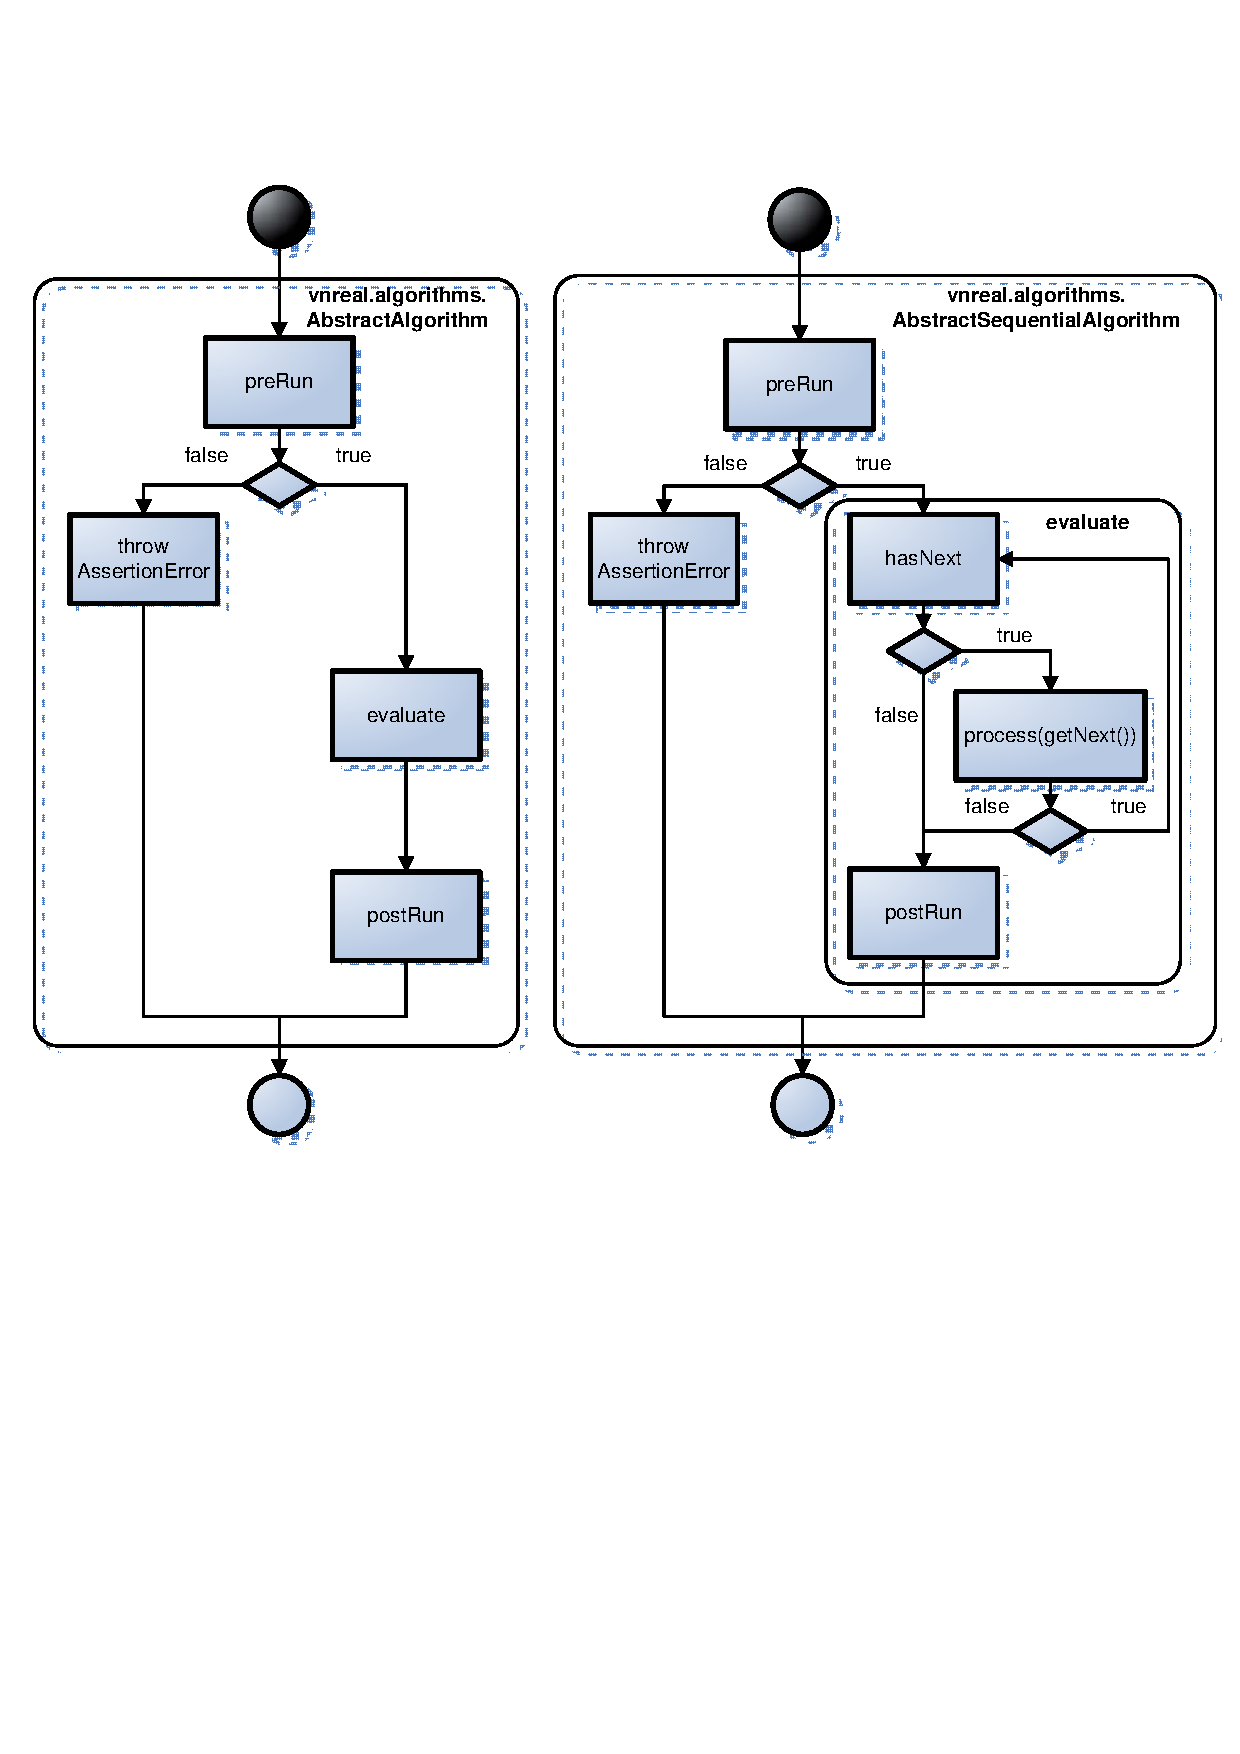
\includegraphics[width=\textwidth]{img/abstractAlgorithms.pdf}
	\end{center}
	\caption{Behaviour of \texttt{AbstractAlgorithm} and \texttt{AbstractSquentialAlgorithm} }
	\label{fig:abstractAlgorithms}
\end{figure}
\item \texttt{vnreal.algorithms.AbstractRevokableSequentialAlgorithm} additionally provides an abstract \textsl{revoke} method
\item Basic algorithmic principle
\begin{enumerate}
	\item The algorithm gets a \texttt{vnreal.network.NetworkStack} which consists of
	\begin{itemize}
		\item a \texttt{vnreal.network.substrate.SubstrateNetwork} with resources
		\item a list of \texttt{vnreal.network.virtual.VirtualNetwork} with demands
	\end{itemize}
	\item The algorithm performs the VNM and VLM by search for resources that are able to fulfill the given demands
\end{enumerate}
\end{itemize}



\subsection{Example}
The package \textit{vnreal.algorithms.samples} contains experimental algorithms, like the \texttt{Simple\-Dijkstra\-Algorithm}. This exemplary algorithm performs
\begin{itemize}
	\item an arbitrary virtual node mapping (choosing the node mapping in an arbitrary way among the substrate nodes accomplishing the virtual node demands), 
	\item the virtual link mapping is implemented by connecting each pair of mapped virtual nodes by the shortest path in the substrate network calculated using the Dijkstra algorithm.
\end{itemize}
The first part of the class \texttt{SimpleDijkstraAlgorithm} implementation looks like
\begin{lstlisting}
public final class SimpleDijkstraAlgorithm extends AbstractSequentialAlgorithm<VirtualLink> {
	private final NetworkStack stack;//Set of networks including the substrate network and the set of virtual network requests.
	private Iterator<? extends Network<?, ?, ?>> curNetIt;//Iterator over the set of virtual network requests
	private Iterator<VirtualLink> curIt;//Interator over the set of virtual links of a virtual network request 
\end{lstlisting}
This is the \textsl{hasNext} function of this algorithm which simply updates the iterator over the set of virtual network requests. If one virtual network requesthas already been served, it moves the \textsl{curNetIt} to the next virtual network request and updates \textsl{curNetIt} iterator. If there is no more virtual network requests it returns false. 
\begin{lstlisting}
@Override
protected boolean hasNext() {
	if (curIt == null || !curIt.hasNext()) {
		if (curNetIt.hasNext()) {
			Network<?, ?, ?> tmp = curNetIt.next();
			if (tmp instanceof SubstrateNetwork)
				tmp = curNetIt.next();
			curIt = ((VirtualNetwork) tmp).getEdges().iterator();
			return hasNext();
		} else
			return false;
	} else
		return true;
}
\end{lstlisting}
The \textsl{getNext} method returns the following virtual link that will be mapped in the process method. To see the example code in detail  take a look at the \textit{vnreal.algorithms.samples} package. 
\begin{lstlisting}
@Override
protected VirtualLink getNext() {
	if (!hasNext())
		return null;
	else
		return curIt.next();
}
\end{lstlisting}
\section{Easily Reusing Existing Node/Link Mapping Algorithms}
The \texttt{SimpleDijkstraAlgorithm} is an example of how to implement an algorithm to solve the virtual network mapping, 
when the virtual link and node mapping are performed as a single stage. 
However, most of the algorithms to solve the VNE are divided in two stages:
\begin{enumerate}
	\item Virtual node mapping (performed in first place) and
	\item Virtual link mapping (performed in second place).
\end{enumerate}
To facilitate the task of implementing a VNE algorithm, the abstract \texttt{vnreal.algorithms. GenericMappingAlgorithm} class should be used.

The \texttt{GenericMappingAlgorithm} class takes two parameters: NodeMapping and LinkMapping. 
These need to be derived from the two classes \texttt{vnreal.\-algorithms.\ AbstractNodeMapping} and \texttt{vnreal.algorithms.AbstractLinkMapping}, respectively. 
In this way, the node mapping and link mapping stages can be implemented independently of each other. 
This has an important advantage: the node and link mapping stages of different algorithms can be combined, 
which may leads to different results.

GenericMappingAlgorithm works by processing each time a different virtual network 
request so the \textsl{getNext()} method returns a virtual network request. 
The \textsl{process(VirtualNetwork p)} method, 
receive this virtual network request and performs node mapping and link mapping stages. 
If at least one of them were not successful, 
all the mappings over that virtual network are undone and the method finishes 
(without realizing the mapping of that network); if they were both successful, 
the method finishes. 
The flow chart in figure \ref{fig:genericMappingAlgorithm} of the algorithm is shown next.
Different methods of \texttt{AbstractNodeMapping} and \texttt{AbstractLinkMapping} are described after the figure.
\begin{figure}[h]
  \begin{center}
		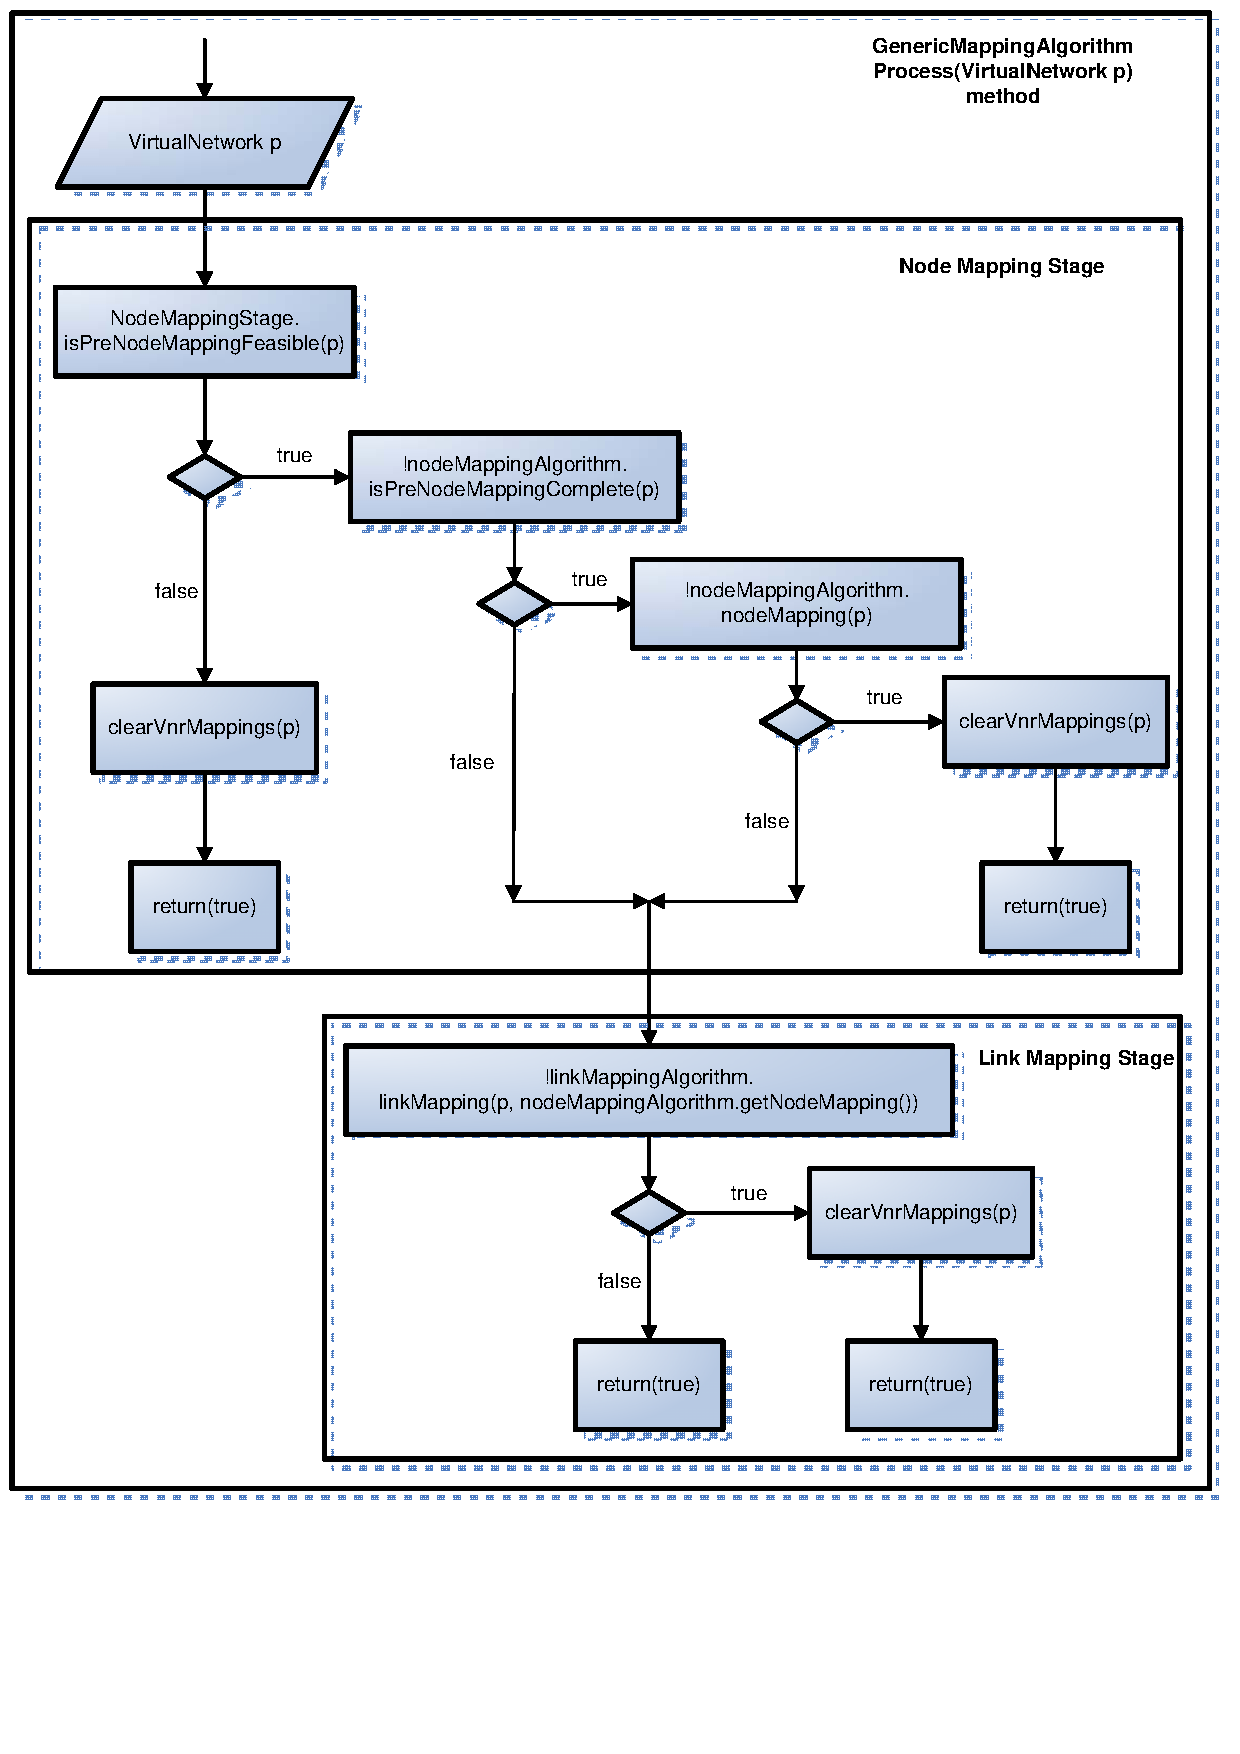
\includegraphics[width=\textwidth]{img/genericMappingAlgorithm.pdf}
	\end{center}
	\caption{Behaviour of \texttt{GenericMappingAlgorithm} }
	\label{fig:genericMappingAlgorithm}
\end{figure}

To implement a new algorithm that has both,
node and link mapping stage, two classes need to be implemented. 
Node mapping class that extends from \texttt{AbstractNodeMapping} and the link mapping class that extends from \texttt{AbstractLinkMapping}.


\subsection{AbstractNodeMapping}
Now let's check the \textbf{methods and variables} of \texttt{AbstractNodeMapping}:
\begin{lstlisting}
public abstract class AbstractNodeMapping {
	protected Map<VirtualNode, SubstrateNode> nodeMapping;
	private List<VirtualNode> unmappedvNodes;
	private List<SubstrateNode> unmappedsNodes;
	protected List<SubstrateNode> mappedsNodes;
\end{lstlisting}
The previous global variables have the following meaning:
\begin{itemize}
	\item \textsl{nodeMapping}: It is a list of Map type that contains the mapping of each \texttt{VirtualNode} 
	to its corresponding \texttt{SubstrateNode} after the node mapping is realized. 
	This variable should be updated while mapping is being performed.
	\item \textsl{unmappedvNodes}: It is a list with the virtual nodes that have not been mapped for the current virtual network request, after a predefined node mapping have been performed. ALEVIN supports the possiblity of predefining the mapping of a set of virtual nodes (possibly all) into its corresponding substrate nodes.
	\item \textsl{unmappedsNodes}: It is a list with the substrate nodes that have not been mapped, for the current virtual network request, after a predefined node mapping have been performed.
	\item \textsl{mappedsNodes}: It is a list with the substrate nodes that have been mapped, for the current virtual network request, performing the predefined node mapping.
\end{itemize}



\begin{lstlisting}
public boolean isPreNodeMappingFeasible(VirtualNetwork vNet)
\end{lstlisting}
ALEVIN supports a resource/demand called id in nodes: 
In this way it is possible to realize a predefined node mapping before the algorithm runs, it is enough to assign in the \texttt{IdDemand} of the virtual nodes the \texttt{IdResource} of the substrate nodes that are chosen to realize the mapping. 
The \textsl{isPreNodeMappingFeasible} method is responsible of realizing this predefined mapping and ensures that the resources of the mapped substrate nodes are enough to cover the demands of the virtual nodes. 
The method returns a false value if the mapping could not be performed. 
This method is already implemented in \texttt{AbstractNodeMapping} and used in \texttt{GenericMappingAlgorithm}. 
After the method is performed, \textsl{nodeMapping}, \textsl{unmappedvNodes}, \textsl{unmappedsNodes} and \textsl{mappedsNodes} are updated.



\begin{lstlisting}
public boolean isPreNodeMappingComplete() {
	return unmappedvNodes.isEmpty();
}
\end{lstlisting}
The method \textsl{isPreNodeMappingComplete()} checks if in the predefined node mapping stage the virtual node mapping has been performed completely or not. It is complete if all virtual nodes have been mapped, in this case no virtual node mapping should be performed. This method is already implemented in \texttt{AbstractNodeMapping} and used in \texttt{GenericMappingAlgorithm}.

\begin{lstlisting}
protected abstract boolean nodeMapping(VirtualNetwork vNet);
\end{lstlisting}
The \textsl{nodeMapping} method is the most important method of the class. 
\textbf{This method} is the one that has to be implemented in a new class (extending \texttt{AbstractNodeMapping}). 
It is important to know, when implementing this method, that probably a predefined mapping has been performed 
and some virtual nodes of the virtual network request have already been mapped (take into account \textsl{nodeMapping}, 
\textsl{unmappedvNodes}, \textsl{unmappedsNodes} and \textsl{mappedsNodes} variables). 
After the \textsl{nodeMapping} has been performed, the \textsl{nodeMapping} variable should be updated and the method should return a boolean value (true if the node mapping was successful, false otherwise).
To see some implementations of the \textsl{nodeMapping()} method, please go to \textit{vnreal.algorithms.nodemapping} package.




\subsection{AbstractLinkMapping}
Now let's check the \textbf{methods and variables} of \texttt{AbstractLinkMapping}:
\begin{lstlisting}
public abstract class AbstractLinkMapping {
	protected int processedLinks, mappedLinks;
\end{lstlisting}
The \texttt{AbstractLinkMapping} variables \textsl{processedLinks} and \textsl{mappedLinks} are used to update the progress bar of the algorithm. 
When a virtual link is being mapped, \textsl{processedLinks} should be incremented by 1, 
and when it have been already mapped, \textsl{mappedLinks} should also be incremented by 1.



\begin{lstlisting}
protected abstract boolean linkMapping(VirtualNetwork vNet,Map<VirtualNode, SubstrateNode> nodeMapping);
\end{lstlisting}
The main method of the \texttt{AbstractLinkMapping} class is the abstract \textsl{linkMapping} method. 
\textbf{This method} is the one that has to be implemented in a new class (extending \texttt{AbstractLinkMapping}). 
The input is the virtual network request and the already performed \textbf{node mapping}. 
The output of the method should be a boolean true if the node mapping was successful, false otherwise).


\subsection{Required GUI adoptions}
If you want your new algorithm to appear in the GUI, simply extend the class \texttt{vnreal. gui.menu.AlgorithmsMenu}.

\section{Adding of New Pair of Resource/Demand Types}

\subsection{Overview}
\begin{itemize}
	\item All resource types are derived from \texttt{AbstractResource}
	\item Resources may only be added to the entities of the \texttt{SubstrateNetwork}
	\item The \texttt{SubstrateNetwork} consists of \texttt{SubstrateLinks} and \texttt{SubstrateNodes}
	\item All demand types are derived from \texttt{AbstractDemand}
	\item Demands may only be added to the entities of a \texttt{VirtualNetwork}
	\item A \texttt{VirtualNetwork} consists of \texttt{VirtualLinks} and \texttt{VirtualNodes}
\end{itemize}
We use the \textbf{Visitor pattern}\footnote{See \href{http://en.wikipedia.org/wiki/Visitor_pattern}{http://en.wikipedia.org/wiki/Visitor\_pattern}} 
and \textbf{Adapter pattern}\footnote{See \href{http://en.wikipedia.org/wiki/Adapter_pattern}{http://en.wikipedia.org/wiki/Adapter\_pattern}}  to avoid
\begin{itemize}
	\item casts to concrete demand/resource classes,
	\item the use of Java's instanceof as far as possible.
\end{itemize}
\textbf{N.b.: } We use these design pattern in an entangled way.
\begin{itemize}
	\item A resource is a visitor for a demand providing the occupy and free visitors
	\item A demand is a visitor for a resource providing the accepts and fulfills visitors
	\item Do not get confused about this.
	\item Every Resource and Demand has a name. When you create a clone (with \textsl{getCopy()}) you have to copy the name over to the clone. 
	So that the equals()-Method can do matches with clones.
	\item If you don't provide a name, the name is set to \textbf{NameOfOwner\_this.hashCode()}
\end{itemize}


\subsection{About the visitor pattern}
Normally the visitor pattern is used to be able to add new operations to an existing object structure, 
without altering every single object. 
The operations get encapsulated in visitors, 
which then visit the objects and interacts with them. 
The object only have to provide a simple interface to accept visitors.
Here we already know all operations we need (free, occupy, accepts, fulfills), 
but want to be able to add new resource / demand pairs to our network, e.g. new objects, 
which then can handle all upcoming resource / demand requests.

%TODO: Need to add the Constructor Parameters
\subsection{Constraints}
For ALEVIN's \textbf{XML exchange format}\footnote{See SVN\_base/src/XML/Alevin.xsd}, resource and demand classes need to meet the following constraints
\begin{itemize}
	\item The constraint classes must implement one or both of the \texttt{INodeConstraint}, \texttt{ILinkConstraint} interfaces. This shows whether the Constraint is applicable to nodes, links or both.
	\item For each parameter that shall be included in the exchange format, a getter and a setter method \textbf{must be declared and  annotated} with @ExchangeParameter 
	\begin{itemize}
		\item Getters are required for export
		\item Setters are required for import
	\end{itemize}
	\item The parameters for these methods \textbf{must not} be simple types (int, double) but classes 
	such that it can be used via Java Reflection
	\begin{itemize}
		\item N.B.  Currently, the exchange format supports the following types: Integer, Double, String, Boolean and ArrayList<String>
	\end{itemize}
	\item Resources
	\begin{itemize}
		\item Getter methods must be named according to the following pattern: get + <parameter name>
		\item Setter methods must be named according to the following pattern: set + <parameter name>
	\end{itemize}
	\item Demands
	\begin{itemize}
		\item Getter methods must be named according to the following pattern: getDemanded + <parameter name>
		\item Setter methods must be named according to the following pattern: setDemanded + <parameter name>
	\end{itemize}
	\item Constructors
	\begin{itemize}
		\item It's suggested that you use a default constructor only with the owner as parameter.
		\item If you need to have additional parameter you need to add the @ConstructionParameter annotation
		\item If you have more than one parameter, the parameterName and parameterGetter have to be in the right order.
		\begin{lstlisting}
@AdditionalConstructParameter(
		parameterNames = {"sNetwork"},
		parameterGetters = {"getsNetwork"}
)
public final class IdResource extends AbstractResource implements
		INodeConstraint {
	private String id;
	private final SubstrateNetwork sNetwork;


	public IdResource(Node<? extends AbstractConstraint> owner, SubstrateNetwork sNetwork) {
		super(owner);
		this.sNetwork = sNetwork;
	}
	...
		\end{lstlisting}
	\end{itemize}
\end{itemize}


\subsection{Procedure}
To add the new demand type \texttt{MyNewDemand} and the corresponding resource type \texttt{MyNewResource} perform the following steps: 
\begin{enumerate}
	\item Add dummy methods to
	\begin{itemize}
		\item \textsl{vnreal.demands.DemandVisitorAdapter }
		\begin{lstlisting}
public boolean visit(MyNewDemand req) {
  return false;
}
		\end{lstlisting}
		\item \textsl{vnreal.resources.ResourceVisitorAdapter }
			\begin{lstlisting}
public boolean visit(MyNewResource req) {
  return false;
}
		\end{lstlisting}
	\end{itemize}
	\item Create a new class \texttt{MyNewResource} in package \textit{vnreal.resources} extending \texttt{AbstractResource}
	\item Create a new class \texttt{MyNewDemand} in package \textit{vnreal.demands} extending \texttt{AbstractDemand}
	\item Implement all abstract methods (imitate existing code, like \texttt{IdDemand} and \texttt{IdResource}) 
\end{enumerate}

\section{Mapping of Demands on Resources}

\subsection{How Demands are Mapped to Resources and Vice Versa}
Mappings between demands and resources are established by the mapping algorithms. 
For each demand, the algorithms determine the resources fulfilling it.

To create a mapping between a demand an a resource the following steps ar needed:
\begin{enumerate}
	\item The resource must accept the demand. In this step, it is determined if the resource and demand are compatible.
	\item The resource must fulfill the demand. This assures that the resource is sufficient for the demand's requirements.
	\item Finally, the demand occupies the resource. In this step, the free capacity of the resource is reduced and a mapping between the two constraints is created.
\end{enumerate}
To remove an existing mapping, the demand must free the occupied resource.


\subsection{How to Deal with Demand-Resource Mappings}
\begin{itemize}
	\item Access
	\begin{itemize}
		\item Get occupied resource from a demand: 
		\begin{lstlisting}
AbstractDemand d;
for (vnreal.mapping.Mapping m : d.getMappings()) {
  AbstractResource r = m.getResource();
�
  // ...
}
		\end{lstlisting}
		\item Get occupying demands of a resource: 
			\begin{lstlisting}
AbstractResource r;
for (vnreal.mapping.Mapping m : r.getMappings()) {
  AbstractDemand d = m.getDemand();
�
  // ...
}
		\end{lstlisting}
		\item Removal
		\begin{lstlisting}
AbstractDemand d;
AbstractResource r;
�
d.getMapping(r).unregister(); // unlinks both elements		
		\end{lstlisting}
	\end{itemize}
\end{itemize}


\subsection{Example for occupying and freeing resources}
To occupy a resource for a virtual network, the \textsl{occupy()} method of the corresponding Demand gets called. 
The \textsl{occupy()} method retrieves the occupy visitor from the Resource, which then visits the Resource.

First it checks if the Resource is able to fulfill the Demand by calling the \textsl{fulfills()} method of the Resource. 
The \textsl{fulfills()} method retrieves the fulfills visitor from the Demand, which then visits the Resource and 
returns if it is able to fulfill the demand. 
This result gets forwarded to the occupy visitor, which then creates a new Mapping to occupy the demanded resource. 
The Mapping registers itself at the Demand and the Resource.

At last the occupy visitor returns if the resource occupation was successful. 
This results gets forwarded to the caller of the \textsl{occupy()} method.


\textbf{Missing Pucture... occupy pdf}

To free a resource, which is no longer needed, the \textsl{free()} method of the corresponding Demand gets called. 
The \textsl{free()} method retrieves the free visitor from the Resource, which then visits the Resource.

The free visitor takes the corresponding mapping and advises it to unregister itself from the Demand and the Resource. If this was successful, the Resource is freed and the result gets forwarded to the Demand and from there to the caller of the \textsl{free()} method.

\textbf{Missing Pucture... free pdf}
\section{Test Generation, Running and Plotting}

\subsection{The Basic concept}
The test-system uses the classes \texttt{TestRun} and \texttt{TestSeries}, which can be found in package \textit{test}, as the basis for handling the data.
A \texttt{TestRun} represents one test with the parameters, results and the complete \texttt{Scenario}.
The \texttt{TestSeries} consists of at least one \texttt{TestRun}, a name and the "TestGenerator" which created the tests.

The test-system consists of two parts.
The first part includes classes which are generating tests with parameters or working with them.
This category contains the \texttt{TestRun}, \texttt{TestSeries}, \texttt{XMLImporter}, \texttt{XMLExporter}, \texttt{PlainFileExporter}, 
\texttt{Plotter} and the "TestGenerators". 

A "TestGenerator" which is an implementation of \texttt{AbstractTestGenerator}, creates the \texttt{TestSeries} with all necessary \texttt{TestRun}s. 
The implementation sets the class of the "TestRunner" which will run the Tests, name of the test-series, class of the generator and the number 
runs for one distinct parameter set.
For use in parameters the types \texttt{Double} and \texttt{String} are allowed.
The followig arrays for are already predefined in \texttt{AbstractTestGenerator}:
\begin{lstlisting}
public static final Double[] numSNodesArray = {100d};
public static final Double[] numVNetsArray = {5d};
protected static final Double[] numVNodesPerVNetArray = {10d};
public static final Double[] alphaArray = {0.5};
public static final Double[] betaArray = {0.5};
\end{lstlisting}
If it's necessary, it's possible to redefine them.


The second part contains classes which execute the tests.
A "TestRunner" runs the different \texttt{TestRun}(s) contained in the given \texttt{TestSeries}.
The implementation of a "TestRunner" sets the "SeedGenerator", "NetworkGenerator" and "ResourceGenerator(s)" and "DemandGenerator(s)".
All these generators may need to contain different parameters, if a \texttt{TestRun} is lacking a necessary parameter an error is thrown.
The "SeedGenerator" is optional, but some other generators rely on it, which leads to an error.
The "TestRunner" may run tests in a given number of parallel running threads, this may lead to wrong results, because some
algorithms are not thread-safe and using static data structures.


\textbf{UML Missing here}




\subsection{Running Tests}
To run a test, it's necessary to create a \texttt{TestSeries}. 
This can be done by using a "TestGenerator" or by importing an existing \texttt{TestSeries} using the \texttt{XMLImporter}.

When using a "TestGenerator" it's necessary to create an implementation of the \texttt{Abstract\-Test\-Generator}.
In the constructor there is a need to call the super-constructor and initialize the list of parameters \textsl{mParams}.
Each entry contains a name and an array of values, which can have \texttt{Double} or \texttt{String} as data type.
The name may contain a "marker", in this case "S1" (see exmplate below). 
If a name contains a marker these parameter will be synchronized which means they will be rotated together in one step.

\begin{lstlisting}
public class ExampleTestGenerator extends AbstractTestGenerator {
	protected static final Double[] numVNodesPerVNetArray = { 5d, 10d };
	public static final Double[] numVNetsArray = { 20d, 4d };
	public static final Double[] kShortestPath = { 3d };
	public static final Double[] cpu_min = { 10d, 100d };
	public static final Double[] cpu_max = { 100d, 200d };
	
	public ExampleTestGenerator(String seriesName) {
		super(ExampleTestRunner.class, seriesName, "tests.scenarios.example.ExampleTestGenerator", 30);
		
		mParams = new ArrayList<SimpleEntry<String, Object[]>>();
		//S1 is a marker, which lets these parameters treated in one round
		mParams.add(new SimpleEntry<String, Object[]>("Waxman_alpha", alphaArray));
		mParams.add(new SimpleEntry<String, Object[]>("Waxman_beta", betaArray));
		mParams.add(new SimpleEntry<String, Object[]>("SNetSize", numSNodesArray));
		mParams.add(new SimpleEntry<String, Object[]>("NumVNodesPerNet", numVNodesPerVNetArray));
		mParams.add(new SimpleEntry<String, Object[]>("NumVNets", numVNetsArray));
		//S1 is a marker, which lets these parameters treated in one round: (min,max) := (10,100), (100,200)
		mParams.add(new SimpleEntry<String, Object[]>("S1:Min_CPU", cpu_min)); //For CPU generators
		mParams.add(new SimpleEntry<String, Object[]>("S1:Max_CPU", cpu_max)); //For CPU generators
	}
}
\end{lstlisting}
Now it is possible to create an object of the \texttt{ExampleTestGenerator} and generate the \texttt{TestSeries} calling the method
\textsl{generateTests()}.
In the example 240 \texttt{TestRun} objects are created, for any possible combination of parameters, 8 in this case with 30 distinct runs for each.

The next step is to run the tests, it is necessary to implement a "TestRunner" using the \texttt{AbstractTestRunner}.
\begin{lstlisting}
public class ExampleTestRunner extends AbstractTestRunner {
	public ExampleTestRunner(XMLExporter exporter) {
		super(new StandardSeedGenerator(), new FixedWaxmanNetworkGenerator(), true, exporter);
		
		//Set generator for resources
		mResGens.add(new FixedCpuResourceGenerator()); //needs parameters: Min_CPU and Max_CPU
		mResGens.add(new IdResourceGenerator());
		
		//Set generator for demands
		mDemGens.add(new FixedCpuDemandGenerator()); //needs parameters: Min_CPU and Max_CPU
		
		//Set Metrics
		mMetrics.add(new AcceptedVnrRatio());
		mMetrics.add(new RejectedNetworksNumber());
	}

	@Override
	protected IAlgorithm prepareRunnerStage2(TestRun tr) {
		NetworkStack ns = tr.getScenario().getNetworkStack();
		IAlgorithm algo = new SubgraphIsomorphismStackAlgorithm(ns,
				new AdvancedSubgraphIsomorphismAlgorithm(false));
		return algo;
	}
}
\end{lstlisting}

The super constructor will be called with the following parameters:
\begin{enumerate}
	\item "SeedGenerator" based on \texttt{AbstractSeedGenerator}, can be null.
	\item "NetworkGenerator"  based on \texttt{AbstractNetworkGenerator}
	\item \texttt{boolean} which says whether the links should be bidirectional or not
	\item \texttt{XMLExporter} which will export the results
\end{enumerate}
Then the generators for "Resources", "Demands" and the metrics need to be set.
At last it's necessary to implement the method \textsl{prepareRunnerStage2()} which creates and prepares the algorithm which is used for the tests.

The last step is to run the tests, done by a simple main-class
\begin{lstlisting}
public class ExampleMain {

	public static void main(String[] args) {
		//Create the TestGenerator and generate the TestSeries
		ExampleTestGenerator gen = new ExampleTestGenerator("Example TestSeries");
		TestSeries series = gen.generateTests();
		
		//Create the XMLExporter which is used, which doesn't export the Networks
		XMLExporter exporter = new XMLExporter("Result.xml", series.getTestSeriesName(), 
		series.getTestGenerator(), false);
		
		//Create the TestRunner and run the tests in 5 parallel threads
		GeneratorTestRunner run = new GeneratorTestRunner(exporter);
		run.runAllTest(series.getAllTestRuns(), 5);
	}
}
\end{lstlisting}




\subsection{Plotting}
The class \texttt{Plotter} in package \textit{plot} provides a simple method to filter the data and create plots in 2D and 3D.
It's possible to filter the data using \textsl{applyFilter*} methods.
Each filter method need to have the following parameters:
\begin{enumerate}
	\item Name of the parameter or metric as String
	\item (Start) Value of the parameter with type \texttt{Double} or \texttt{String} (String only for \textsl{applyFilterEqual} and \textsl{applyFilterNotEqual}
	\item End Value of the parameter with type \texttt{Double} (Only nneded in range filters)
\end{enumerate}
If the statement is true, the test will removed from the list.

The output-methods always need to have a directory name, in which the results will be plotted and the files are named after the metric which is plotted.
A 2D plot \textsl{output2d} need to have one parameter and a 3D plot \textsl{output3d} need to have two parameters.
The ordering is based on the given parameter(s).
\\
\textbf{Be aware:} At the moment it isn't possible to use \texttt{String} based parameters.

\begin{lstlisting}
public class ExamplePlotMain {
	public static void main(String[] args) {
		TestSeries series2 = XMLImporter.importResults("Result.xml");
		
		Plotter p = new Plotter(series2);
		p.applyFilterEquals("AcceptedVnrRatio", 0.0);
		
		p.output2D("ExamplePlot2d", "NumVNodesPerNet", "AcceptedVnrRatio");
		p.output3D("ExamplePlot3d", "NumVNodesPerNet", "Min_CPU", "AcceptedVnrRatio");
	}
}
\end{lstlisting}



\subsection{Writing a Generator}
To run tests there are different types of generators:
\begin{itemize}
	\item "SeedGenerators" based on \texttt{AbstractSeedGenerator} which are creating seeds for random generators
	\item "NetworkGenerators" based on \texttt{AbstarctNetworkGenerator} which are creating the network stack
	\item "ResourceGenerators" based on \texttt{AbstarctResourceGenerator} which are creating a resource
	\item "DemandGenerators" based on \texttt{AbstarctResourceGenerator} which are creating a demand
\end{itemize}


A generator has always implement the methods \textsl{generate} which contains the logic and \textsl{reset} 
which resets the state if needed and is called before a every new \texttt{TestRun}.
If the generator needs parameters, these are specified in the \texttt{GeneratorParameter} annotation.
The parameter array will filled with these values in order of annotation.
The following values are possible:
\begin{itemize}
	\item "Seed:Seed": Seed from "SeedGenerator" from type \texttt{Double}
	\item "Networks:Networks": The \texttt{NetworkStack}
	\item "TR:ParameterName": The value for the parameter with the name "ParameterName" from \texttt{TestRun} (TR)
	\item "Result:package.ResoureOrDemandGenerator": The result of the \textsl{generate} method of the given and used demand or resource generator
	\item "Method:package.ResoureOrDemandGenerator|getFoo": The result of the non-static \textsl{getFoo} method of the given and in this "TestRunner"' used demand or resource generator
	\item "SMethod:some.package.Class|getBar": The result of the static \textsl{getBar} method of the given class "some.package.Class"
 \end{itemize}

If a parameter is not available or there is an error, an \texttt{Error} is thrown.
\textbf{Be aware:}Due to parallel execution of threads the call of static methods may lead to wrong results!


\begin{lstlisting}
@GeneratorParameter(
		parameters = { "Networks:Networks", "TR:Min_CPU", "TR:Max_CPU", "Seed:Seed"}
		)
public class FixedCpuResourceGenerator extends AbstractResourceGenerator<List<CpuResource>> {

	@Override
	public List<CpuResource> generate(ArrayList<Object> parameters) {
		ArrayList<CpuResource> resList = new ArrayList<CpuResource>();
		
		NetworkStack ns = (NetworkStack)parameters.get(0);
		Integer minCPU = ConversionHelper.paramObjectToInteger(parameters.get(1));
		Integer maxCPU = ConversionHelper.paramObjectToInteger(parameters.get(2));
		Long seed = ConversionHelper.paramObjectToLong(parameters.get(3));
		
		Random random = new Random();
		random.setSeed(seed);
		
		SubstrateNetwork sn = ns.getSubstrate();
		
		for(SubstrateNode n : sn.getVertices()) {
			CpuResource cpu = new CpuResource(n);
			int value = (int) (minCPU + (maxCPU
					- minCPU + 1)
					* random.nextDouble());
			cpu.setCycles((double) value);
			n.add(cpu);
			resList.add(cpu);
		}
		return resList;
	}

	@Override
	public void reset() {}
}
\end{lstlisting}


%\section{Experimental}
%
%Vibrational spectra were recorded in the spectral range from 4000 to 600 cm?1 with a Bruker Equinox 55 FTIR Spectrometer equipped with an MCT detector and diffuse reflectance infrared Fourier transform spectroscopy optics (model DRA-2CO, Harrick Scientific Corp.). The vacuum chamber (model HVC-DR3, Harrick Scientific Corp.) was connected to a standard flow system (Figure 1). Spectra were recorded at a resolution of 4 cm$^{-1}$. 100 scans were averaged for each spectrum resulting in a time resolution of one minute. In order to improve the time resolution for experiments with high NO$_2$ concentrations during the initial phase only 50 scans were averaged.
%
%
%%\begin{landscape} %in case a table becomes to big this rotates it, uncheck also \end{landscape} and lscape package in the preferences
	%\begin{table}
		%\caption[Substrate matrix 1]{\rule[-2mm]{0mm}{0mm}{Physical properties of the tested substrate samples}}
		%\begin{tabular}{@{}*{8}l@{}} \toprule \addlinespace[0.1em]
%
      %No.  &  Supplier  &  Material  &    Sample  &    Length  &  Identifier  &      Mass  &       Mass \\
%
           %&            &            &            &       /cm  &              &      Mass  & /g$^{a)}$ \\
%
%\cmidrule{1-8} % &            &            &            &            &            &            &            \\
%
         %1 &        SST &     Galaxy &  warp unit &         15 &   \color{red}ncc1701e &     1927.6 &     1920.2 \\
%
         %2 &        SST & Constellat. &  warp unit &       14.9 &   11016910 &    ---     &    ---     \\
%
         %3 &        SST &  Prototype &        ops &         15 &  302/09     &    107.766 &    107.771 \\
%
         %4 &    KEmpire &        BoP &  warp unit &       15.1 &     c836f5 &    129.711 &    129.711 \\
%
         %5 &    KEmpire &        BoP &        ops &       15.3 &     c836f6 &     131.65 &    139.656 \\
%
         %6 &    KEmpire &  AC Mullite   &    core    &        3.2 &     c836f7 &      9.896 &      9.889 \\
%
         %7 &    REmpire &  Proptotye &       body &      ---   &   \color{blue}DHC 1703 &    ---     &    ---     \\
%
         %8 &    REmpire &  Proptotye &       body & {\it 15.2} &   DHC 1704 &    ---     &    ---     \\
%
		%\bottomrule
		%\multicolumn{8}{l}{{\footnotesize$^{a)}$After heat test at 2000�K for 5~h}}\\		
	%\end{tabular}
	%\label{tab:matrix_1}
	%\end{table}
%%\end{landscape}
%
%
%\section{Results}
%
%The results for the loss of weight are listed in table~\ref{tab:matrix_1} and in figure~\ref{fig:particle_size}.
%
%Mineral aerosol represents one of the largest mass fractions of the global aerosol. It consists of windblown soil and is produced mainly in the arid areas of our planet, in particular in the great deserts. Its annual production rate is estimated to be in the order of 200 to 5000 Tg. The smaller size fraction (< 20 $mu$m) may be transported over long distances  of up to 5000 km. Mineral aerosol has been considered a nonreactive, hydrophobic surface . Nevertheless, its impact on the atmospheric radiation budget and on the concentration of cloud condensation nuclei (CCN) have been discussed. Recently, its possible role as a surface for heterogeneous reactions has been taken into account. 
%
%%\begin{figure}
%%%	\begin{center}
%%		\includegraphics[width=13cm]{particle_size.pdf}
%%	\end{center}
%%	\caption{Particle size distribution for three different sources.}
%%	\label{fig:particle_size}
%%\end{figure}
%
%\subsection{Modeling Copy2}
%For example, in a recent modeling study Dentener et. al.  calculated that in large areas more than 40\% of the total atmospheric nitrate is associated with mineral aerosol. However, their results still suffer from large uncertainties in the heterogeneous reaction rates. There is also evidence from field measurements for a correlation of the aerosol nitrate content and the aerosol mineral fraction. A correlation between the nitrate mass size distribution and the mineral aerosol distribution has also been reported . 
%\subsubsection{Composition Copy2}
%Mineral aerosol has a complex chemical and mineralogical composition  in which aluminum in the chemical form of alumosilicates contributes 8 \% by mass. For the present investigation alumina has been chosen as model substance. It has a defined chemical composition and mainly because of its relevance as supporting material for catalysts its surface features have been investigated by infrared spectroscopy, and ab initio calculations. Also, the heterogeneous reactions of CFC's with alumina produced by solid-fuel rocket engines have been discussed with regard to stratospheric ozone depletion .
%
%Mineral aerosol represents one of the largest mass fractions of the global aerosol. It consists of windblown soil and is produced mainly in the arid areas of our planet, in particular in the great deserts. Its annual production rate is estimated to be in the order of 200 to 5000 Tg , , . The smaller size fraction (< 20 $mu$m) may be transported over long distances  of up to 5000 km. Mineral aerosol has been considered a nonreactive, hydrophobic surface . Nevertheless, its impact on the atmospheric radiation budget and on the concentration of cloud condensation nuclei (CCN) have been discussed. Recently, its possible role as a surface for heterogeneous reactions has been taken into account. 
%\subsection{Modeling Copy3}
%For example, in a recent modeling study Dentener et. al.  calculated that in large areas more than 40\% of the total atmospheric nitrate is associated with mineral aerosol. However, their results still suffer from large uncertainties in the heterogeneous reaction rates. There is also evidence from field measurements for a correlation of the aerosol nitrate content and the aerosol mineral fraction. A correlation between the nitrate mass size distribution and the mineral aerosol distribution has also been reported. 
%\subsubsection{Composition Cpoy3}
%Mineral aerosol has a complex chemical and mineralogical composition  in which aluminum in the chemical form of alumosilicates contributes 8 \% by mass. For the present investigation alumina has been chosen as model substance. It has a defined chemical composition and mainly because of its relevance as supporting material for catalysts its surface features have been investigated by infrared spectroscopy, and ab initio calculations. Also, the heterogeneous reactions of CFC's with alumina produced by solid-fuel rocket engines have been discussed with regard to stratospheric ozone depletion.
%
\end{document}



